\documentclass[10pt]{article}

% Basic packages
\usepackage[margin=2.5cm]{geometry}
\usepackage{amsmath,amssymb,amsfonts}
\usepackage{graphicx}
\usepackage{booktabs}
\usepackage{multirow}
\usepackage{array}
\usepackage{subcaption}
\usepackage{float}
\usepackage{algorithm}
\usepackage{algorithmic}
\usepackage{hyperref}
\usepackage{xcolor}
\usepackage{listings}
\usepackage{enumitem}
\usepackage{cite}

% Code style
\lstset{
    basicstyle=\ttfamily\small,
    breaklines=true,
    frame=single,
    language=Python
}

% Hyperlink settings
\hypersetup{
    colorlinks=true,
    linkcolor=blue,
    citecolor=blue,
    urlcolor=blue
}

\begin{document}

% ==================== Title Page ====================
\title{\textbf{BGE-Attention: A Probabilistic Prediction Framework\\for Social Media Comment Popularity\\Based on Cross-Attention Mechanism}}

\author{
    Junkai Li\\
    \textit{College of Information Engineering, Zhejiang University of Technology}\\
    \texttt{302023568066@zjut.edu.cn}
}

\date{}

\maketitle

% ==================== Abstract ====================
\begin{abstract}
Social media information ecosystems exhibit typical characteristics of complex adaptive systems, where the generation mechanism of comment popularity embeds ontological uncertainty, revealing fundamental limitations of traditional point estimation paradigms. This paper re-examines the popularity prediction problem from an epistemological perspective, arguing that its essence is the estimation of conditional probability distributions with inherent randomness. Based on this insight, we propose the BGE-Attention probabilistic prediction framework: encoding multi-source texts through the BGE pre-trained model, achieving conditional projection in semantic space via Cross-Attention mechanism; designing a log-scale negative log-likelihood loss function to reconstruct scale invariance in error measurement; and proposing MinHash-based temporal-semantic joint features to construct computable representations of the ``first-mover vs. follower'' effect. Experiments on 270,000 Weibo comments demonstrate that compared to the NGBoost baseline, our method reduces the Mean Prediction Interval Width (MPIW) by six orders of magnitude (from tens of millions to 3.0050), while improving PICP@95\% from 94.30\% to 97.75\%, achieving Pareto optimality between prediction accuracy and uncertainty calibration in social media scenarios for the first time. Code is available at: \url{https://github.com/LJK666666666/LLM_SU7}.

\textbf{Keywords:} Probabilistic prediction; Uncertainty quantification; Pre-trained language models; Cross-attention mechanism; Long-tail distribution modeling
\end{abstract}

% ==================== 1. Introduction ====================
\section{Introduction}

\subsection{Research Background: Popularity Prediction from a Complex Systems Perspective}

Social media has evolved into a typical \textbf{complex adaptive system}: micro-level interaction behaviors of individual users and macro-level propagation patterns of emergent groups are mutually coupled, forming cross-scale nonlinear dynamics\cite{liu2019sentiment}. Comment popularity---as a projection of the ``content-user-platform'' ternary interaction---embeds \textbf{ontological uncertainty} in its generation mechanism: identical semantic content at different temporal positions can produce order-of-magnitude differences in propagation effects. This phenomenon has significant application value for public opinion monitoring\cite{zhang2020brand}, brand management, and content recommendation\cite{wu2019npa}, but also reveals the fundamental limitations of traditional deterministic prediction paradigms.

From an information-theoretic perspective, existing research has fallen into the \textbf{``point estimation trap''}: forcibly mapping the inherently stochastic popularity evolution process to a deterministic numerical space. This not only causes semantic deficiency in prediction confidence but fundamentally conflates the boundaries between \textbf{epistemic uncertainty} (arising from incomplete model knowledge) and \textbf{aleatoric uncertainty} (arising from inherent data randomness).

\subsection{Technical Challenges: Systematic Analysis of Triple Bottlenecks}

Through in-depth analysis of existing methods, we identify three technical bottlenecks constraining prediction performance:

\textbf{(1) Scale distortion effect of loss functions}. Social media data exhibits typical power-law distribution, where a few comments receive massive interactions while most receive sparse engagement. Traditional mean squared error loss shows severe \textbf{dimensional bias} in this scenario: excessive sensitivity to absolute errors for high-popularity samples while systematically underestimating relative errors for low-popularity samples. The essence of this deficiency lies in the failure of Euclidean distance metrics to capture the \textbf{multiplicative noise characteristics} of social media data---prediction errors should be proportional to true values rather than absolute.

\textbf{(2) Decoupling dilemma between semantic representation and context}. Existing text encoding schemes generally adopt naive ``encode-concatenate'' strategies, ignoring the \textbf{conditional dependency structure} between comment semantics and their context (Weibo posts, parent comments, root comments). Such architectures cannot model the phenomenon of ``same comment having vastly different popularity in different contexts,'' essentially constituting systematic omission of \textbf{pragmatic information}.

\textbf{(3) Modeling gap for temporal position effects}. The popularity gap between ``first-mover effect'' and ``follower effect'' reveals a long-neglected prior: \textbf{the interaction between textual similarity and temporal precedence} constitutes a key explanatory variable for popularity prediction. However, the $O(n^2)$ complexity of brute-force text similarity computation makes this feature impractical at scale.

\subsection{Our Contributions: From Tactical Improvements to Paradigm Innovation}

Addressing these challenges, this paper proposes the BGE-Attention probabilistic prediction framework, achieving a \textbf{paradigm shift} from ``point estimation'' to ``distribution prediction.'' Main contributions include:

\begin{enumerate}[leftmargin=*]
    \item \textbf{Prediction paradigm reconstruction}: Proposing the BGE-Attention model with dual prediction heads that simultaneously output mean $\mu(x)$ and standard deviation $\sigma(x)$, achieving joint modeling of predicted values and prediction confidence, explicitly encoding the inherent randomness of prediction targets;
    \item \textbf{Reconstructing scale invariance in loss functions}: Designing a log-scale negative log-likelihood loss function that achieves equal-weight penalization of cross-magnitude prediction errors by mapping error metrics from original space to log space, while constructing an endogenous uncertainty regularization mechanism;
    \item \textbf{Conditional projection in semantic space}: Employing Cross-Attention mechanism to establish conditional mapping between ``comment semantics-context semantics,'' elevating comment representations from ``isolated semantics'' to ``contextualized semantics'';
    \item \textbf{Constructing temporal-semantic joint feature space}: Proposing MinHash-based duplication features that reduce similarity computation complexity from $O(n^2)$ to $O(nk)$, providing computable mathematical expressions for the ``first-mover vs. follower'' effect.
\end{enumerate}

% ==================== 2. Related Work ====================
\section{Related Work}

\subsection{Social Media Popularity Prediction: From Time Series Modeling to Deep Learning}

The research trajectory of social media popularity prediction has undergone paradigm evolution from statistical modeling to deep learning. Early work mainly relied on time series models\cite{yang2011patterns}, predicting final popularity by analyzing propagation temporal features (such as early growth rate, peak time), with theoretical foundations in the \textbf{Matthew effect} of information propagation---content gaining early attention tends to continue receiving attention. Bandari et al.\cite{bandari2012pulse} studied news article sharing prediction, finding that content features and sources significantly impact performance, revealing the \textbf{interaction between content factors and channel factors} in popularity prediction.

In recent years, deep learning methods have achieved significant progress. Deng et al.\cite{deng2020deep} proposed attention-based neural network models to capture complex user-content interactions. However, these methods generally share an \textbf{epistemological limitation}: focusing only on point estimation while ignoring uncertainty modeling in predictions. This paper argues that the essence of popularity prediction is the estimation of \textbf{conditional probability distributions}, and point estimation paradigms cannot express the model's confidence in prediction results.

\subsection{Pre-trained Language Models: From Bag-of-Words to Context-Aware Representations}

Text representation technology has undergone profound transformation from \textbf{symbolic space} to \textbf{continuous vector space}. Traditional TF-IDF and bag-of-words models map text to sparse high-dimensional vectors, failing to capture word order information and semantic relationships. The emergence of pre-trained language models marks a paradigm revolution in NLP: BERT\cite{devlin2019bert} learns bidirectional contextual representations through masked language modeling, while RoBERTa\cite{liu2019roberta} further optimized pre-training strategies.

BGE (BAAI General Embedding)\cite{bge2023} is a text embedding model designed for Chinese, with core innovation in introducing the \textbf{contrastive learning paradigm}---through discriminative training on positive and negative sample pairs, semantically similar texts become closer in embedding space. This paper adopts BGE-base-zh-v1.5 for extracting comment semantic representations and implements \textbf{context-aware semantic fusion} through Cross-Attention mechanism, enabling comment representations to dynamically adapt to their conversational context.

\subsection{Probabilistic Prediction and Uncertainty Estimation: From Point Estimates to Distribution Outputs}

Uncertainty estimation is a research direction with profound theoretical implications in machine learning\cite{gal2016uncertainty}. Bayesian neural networks\cite{blundell2015weight} explicitly model parameter uncertainty by imposing prior distributions on weights; MC Dropout\cite{gal2016dropout} proposes approximating Bayesian inference through multiple stochastic dropouts, but with significant computational overhead.

NGBoost\cite{duan2020ngboost} pioneered the \textbf{natural gradient boosting} technical route, capable of directly outputting prediction distributions by optimizing parameters of conditional distributions (rather than point predictions). However, this method faces two challenges in social media scenarios: (1) loss functions not designed for long-tail distributions; (2) tree models have difficulty effectively utilizing semantic representations from pre-trained language models. Building upon this, our paper proposes \textbf{log-scale loss functions} to reconstruct scale invariance in error metrics, and achieves end-to-end semantic-numerical joint modeling through neural network architectures.

% ==================== 3. Method ====================
\section{Method}

\subsection{Problem Formalization: From Point Estimation to Distribution Estimation}

Given a comment $x$ with its contextual information (associated Weibo post, root comment, parent comment) and statistical features, traditional methods aim to learn the mapping $f: x \mapsto \hat{y}$. This paper redefines the prediction target as estimation of the \textbf{conditional probability distribution} $P(y|x)$.

Based on analysis of social media data distribution characteristics (see Figure~\ref{fig:log_distribution}), we assume that log-transformed popularity follows a normal distribution:
\begin{equation}
\log(y+c) \sim \mathcal{N}(\mu(x), \sigma^2(x))
\end{equation}
where $c$ is a smoothing constant, and $\mu(x)$ and $\sigma(x)$ are the model-predicted \textbf{location parameter} (representing prediction center) and \textbf{scale parameter} (representing prediction uncertainty), respectively. The core insight of this formalization lies in: \textbf{explicitly parameterizing} the uncertainty originally implicit in prediction residuals, enabling the model to output differentiated confidence levels for different samples.

\subsection{Model Architecture: Hierarchical Fusion of Multi-Source Semantics}

The BGE-Attention model architecture proposed in this paper is shown in Figure~\ref{fig:neural_networks}, adopting a \textbf{three-stage ``encode-fuse-predict'' design} with four functional modules.

\begin{figure}[H]
    \centering
    \includegraphics[width=0.9\textwidth]{figures/neural_networks.png}
    \caption{BGE-Attention Model Architecture}
    \label{fig:neural_networks}
\end{figure}

\subsubsection{Text Encoding Module: Independent Representation of Multi-Source Semantics}

BGE-base-zh-v1.5 model is employed for \textbf{independent encoding} of four text types, constructing multi-source semantic representation space:

\begin{itemize}[leftmargin=*]
    \item \textbf{Comment Text}: Content of the current comment, carrying core semantic information;
    \item \textbf{Weibo Text}: Main text of the associated Weibo post, providing \textbf{topic context};
    \item \textbf{Root Comment Text}: Content of the comment chain's root node, reflecting \textbf{discussion mainline};
    \item \textbf{Parent Comment Text}: Content of the directly replied comment, constituting \textbf{conversational context}.
\end{itemize}

Each text yields a 768-dimensional dense vector representation after BGE encoding. \textbf{BGE parameters are frozen} to prevent overfitting on downstream tasks while preserving general semantic knowledge acquired during pre-training.

\subsubsection{Cross-Attention Fusion Mechanism: Context-Aware Semantic Projection}

Distinct from naive vector concatenation strategies, this paper employs Cross-Attention mechanism for \textbf{conditioned semantic fusion}. Using the comment vector as Query and context vectors (Weibo, root comment, parent comment) as Key and Value:

\begin{equation}
\text{Attention}(Q, K, V) = \text{softmax}\left(\frac{QK^T}{\sqrt{d_k}}\right)V
\end{equation}

where $Q \in \mathbb{R}^{1 \times 768}$ is the comment vector, $K, V \in \mathbb{R}^{3 \times 768}$ are context vector matrices, and $d_k = 768$ is the scaling factor. The \textbf{core advantage} of this mechanism lies in: attention weights are \textbf{dynamically computed} based on semantic relevance between the comment and each context, enabling the model to adaptively focus on context information most relevant to the current comment, achieving representation elevation from ``isolated semantics'' to ``contextualized semantics.''

\subsubsection{Dual Prediction Heads: Explicit Modeling of Uncertainty}

The fused semantic vector is concatenated with numerical features and passed through a \textbf{dual prediction head architecture} to output location parameter $\mu$ and scale parameter $\sigma$ separately:

\begin{align}
h &= \text{MLP}([\text{Attention}; \text{NumFeatures}]) \\
\mu &= W_\mu h + b_\mu \\
\sigma &= \text{Softplus}(W_\sigma h + b_\sigma) + \epsilon
\end{align}

where $\epsilon = 10^{-4}$ is a numerical stability constant, and the Softplus function $\log(1+e^x)$ ensures $\sigma > 0$. The design philosophy of dual prediction heads lies in: \textbf{decoupling prediction center from prediction uncertainty}, enabling the model to output narrow confidence intervals for ``high-certainty simple samples'' and wide confidence intervals for ``low-certainty difficult samples.''

\subsection{Log-Scale NLL Loss Function: Reconstructing Scale Invariance}

\begin{figure}[H]
    \centering
    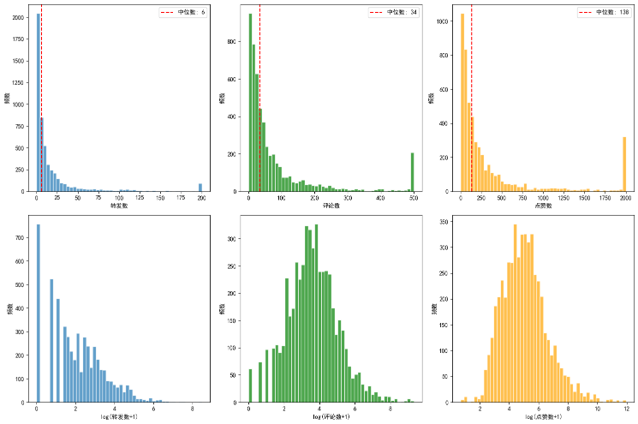
\includegraphics[width=0.9\textwidth]{figures/log_distribution.png}
    \caption{Distribution comparison of popularity data in original scale vs. log scale: original scale shows heavy-tail distribution, log scale approximates normal}
    \label{fig:log_distribution}
\end{figure}

As shown in Figure~\ref{fig:log_distribution}, social media popularity data approximates normal distribution in log scale, providing statistical justification for adopting Gaussian likelihood. This paper employs log-scale negative log-likelihood (NLL) loss:

\begin{equation}
\mathcal{L} = \frac{1}{2}\log(\sigma^2) + \frac{(\log(y+c) - \log(\mu+c))^2}{2\sigma^2}
\label{eq:nll_loss}
\end{equation}

This loss function embodies threefold design wisdom:

\textbf{(1) Scale invariance}: By measuring errors in log space, achieving \textbf{equal-weight penalization of relative errors}. As shown in Table~\ref{tab:smoothing_constant}, $c=10$ reduces the loss ratio between ``predicting 1 when actual is 2'' and ``predicting 110 when actual is 120'' from 4.7 to 1.1, eliminating traditional MSE's excessive focus on small-value samples.

\textbf{(2) Uncertainty regularization}: The $\frac{1}{2}\log(\sigma^2)$ term constructs an endogenous \textbf{confidence penalty mechanism}---if the model outputs overly small $\sigma$ (overconfidence), it will suffer huge second-term loss when prediction deviations occur; conversely, overly large $\sigma$ can reduce the second term but significantly increases the first. This forces the model to seek \textbf{game equilibrium} between ``precise prediction'' and ``honestly acknowledging uncertainty.''

\textbf{(3) Heteroscedastic modeling}: Allowing different samples to have different $\sigma(x)$, enabling the model to output low uncertainty for semantically clear comments (e.g., ``thanks for sharing'') and high uncertainty for semantically ambiguous comments (e.g., ``view image'').

\begin{table}[H]
\centering
\caption{Effect of smoothing constant $c$ on loss function scale sensitivity}
\label{tab:smoothing_constant}
\begin{tabular}{cccc}
\toprule
\textbf{Smoothing Constant} & \textbf{Loss (pred=1, actual=2)} & \textbf{Loss (pred=110, actual=120)} & \textbf{Loss Ratio} \\
\midrule
$c=1$ & $|\log 2 - \log 3| \approx 0.406$ & $|\log 111 - \log 121| \approx 0.086$ & 4.7 \\
$c=10$ & $|\log 11 - \log 12| \approx 0.087$ & $|\log 120 - \log 130| \approx 0.080$ & 1.1 \\
\bottomrule
\end{tabular}
\end{table}

\subsection{Feature Engineering: Systematic Extraction of Multi-Dimensional Signals}

This paper designs four complementary feature categories totaling 17 dimensions, characterizing comment popularity potential from four perspectives: \textbf{user profile, text semantics, topic distribution, and temporal position}.

\subsubsection{Basic Statistical Features and Text Features}

Basic statistical features capture \textbf{user influence} and \textbf{temporal effects}, while text features characterize \textbf{expression intensity} and \textbf{domain relevance}, as detailed in Table~\ref{tab:features}.

\begin{table}[H]
\centering
\caption{Basic Statistical Features and Text Features}
\label{tab:features}
\begin{tabular}{ll}
\toprule
\textbf{Feature Category} & \textbf{Feature Description} \\
\midrule
\multirow{5}{*}{Basic Statistical Features (7D)}
    & User total comments: Historical total comments by comment author \\
    & User verification status: Whether verified account \\
    & Is first-level comment: Distinguishing direct Weibo comments vs. replies \\
    & Weibo comment count: Total comments on associated Weibo post \\
    & Post hour/weekday/is workday: Temporal features \\
\midrule
\multirow{5}{*}{Text Features (6D)}
    & Comment length: Text character count \\
    & Exclamation/question mark count: Emotional and tonal intensity \\
    & Emoji count: Emoji occurrence frequency \\
    & Has hashtag: Whether contains \#topic\# \\
    & Domain keyword count: Xiaomi automotive keyword frequency \\
\bottomrule
\end{tabular}
\end{table}

\subsubsection{LDA Topic Features}

LDA topic model\cite{blei2003latent} is employed for \textbf{latent semantic analysis} of comment texts, mapping high-dimensional word space to low-dimensional topic space. Each comment is assigned to its highest-probability topic as a categorical feature (1D). This feature captures comment \textbf{topical tendency}---different topics (e.g., ``product discussion,'' ``after-sales feedback,'' ``competitor comparison'') have different interaction potential.

\subsubsection{Duplication Features: Constructing Temporal-Semantic Joint Space}

\begin{figure}[H]
    \centering
    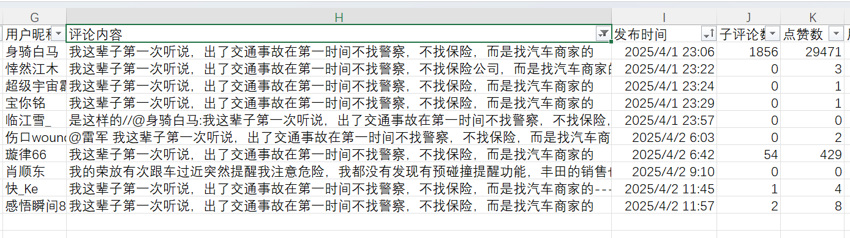
\includegraphics[width=0.9\textwidth]{figures/duplicate_find.png}
    \caption{Comment text duplication patterns: Same text posted multiple times at different timestamps}
    \label{fig:duplicate_find}
\end{figure}

\begin{table}[H]
    \centering
    \caption{Popularity difference between first posts and follower posts: Quantitative evidence of first-mover effect}
    \label{tab:12compare}
    \begin{tabular}{ccc}
        \toprule
        \textbf{Post Order} & \textbf{Mean Reply Count} & \textbf{Mean Like Count} \\
        \midrule
        First Post & 2.24 & 15.95 \\
        Follower Post & 0.17 & 1.13 \\
        Ratio & 13.5$\times$ & 14.2$\times$ \\
        \bottomrule
    \end{tabular}
\end{table}

As shown in Figure~\ref{fig:duplicate_find} and Table~\ref{tab:12compare}, when text is duplicated, first-posted comments receive popularity \textbf{over an order of magnitude higher} than follower comments. This ``first-mover effect'' reveals a long-neglected prior in popularity prediction: \textbf{the interaction between temporal position and text content} is a key explanatory variable. To model this temporal dependency, this paper proposes duplication features based on Jaccard similarity and MinHash algorithm.

\paragraph{Jaccard Similarity: Set-Theoretic Text Similarity Measure}
Given two sets $A$ and $B$, Jaccard similarity is defined as the ratio of intersection to union:
\begin{equation}
J(A, B) = \frac{|A \cap B|}{|A \cup B|}
\end{equation}
Its range is $[0, 1]$, possessing \textbf{symmetry} and \textbf{triangle inequality} properties. Compared to Euclidean distance or cosine similarity, Jaccard similarity is insensitive to set sizes, making it more suitable for measuring similarity of variable-length texts.

\paragraph{N-gram Text Representation: Mapping from Strings to Sets}
Comment texts are converted to character-level N-gram sets, establishing mapping from \textbf{sequence space to set space}. For text $T$, its N-gram set is defined as:
\begin{equation}
\text{Ngram}(T, n) = \{T[i:i+n] | i = 0, 1, ..., |T|-n\}
\end{equation}
This paper adopts $n=3$ (trigrams), e.g., the 3-gram set of ``hello world'' is \{``hel'', ``ell'', ``llo'', ...\}. Character-level N-grams have \textbf{stronger robustness} than word-level representations---no tokenization required, with tolerance for spelling variants and neologisms.

\paragraph{MinHash Signature Algorithm: Probabilistic Approximate Nearest Neighbor Retrieval}
Direct Jaccard similarity computation has time complexity $O(|A| + |B|)$, requiring $O(n^2)$ computations for pairwise comparison of $n$ comments, infeasible at large scale. MinHash algorithm\cite{broder1997resemblance} achieves approximate computation through \textbf{Locality Sensitive Hashing (LSH)}.

Given hash function $h$, the MinHash value of set $S$ is defined as the minimum hash value among elements in $S$:
\begin{equation}
h_{\min}(S) = \min_{s \in S} h(s)
\end{equation}

The \textbf{core theoretical guarantee} of MinHash is: for uniformly random hash function $h$, the probability that two sets have equal MinHash values exactly equals their Jaccard similarity:
\begin{equation}
P(h_{\min}(A) = h_{\min}(B)) = J(A, B)
\end{equation}

This equation \textbf{transforms set operations into probability estimation}. To improve estimation accuracy, $k$ independent hash functions $\{h_1, h_2, ..., h_k\}$ generate signature vectors:
\begin{equation}
\text{Sig}(S) = [h_{1,\min}(S), h_{2,\min}(S), ..., h_{k,\min}(S)]
\end{equation}

Jaccard similarity between two sets is estimated through \textbf{Hamming similarity} of signature vectors:
\begin{equation}
\hat{J}(A, B) = \frac{|\{i : \text{Sig}(A)[i] = \text{Sig}(B)[i]\}|}{k}
\end{equation}

This paper adopts $k=128$ hash functions. By the central limit theorem, the estimation error standard deviation is $O(1/\sqrt{k}) \approx 0.088$, achieving balance between efficiency and accuracy.

\paragraph{Sliding Window Optimization: Balancing Temporal Locality and Global Coverage}
To further reduce computational overhead, a \textbf{sliding window mechanism} is employed: only searching for similar texts within the most recent $W=10000$ comments, while maintaining a global TopK dictionary recording high-frequency duplicate texts. This design is based on the \textbf{temporal locality assumption}---follower comments typically appear within a short time window after first posts. Three features are ultimately generated:
\begin{itemize}[leftmargin=*]
    \item \textbf{Temporal order index}: Comment's temporal order in data, capturing \textbf{position prior};
    \item \textbf{Maximum similarity}: Maximum Jaccard similarity with historical comments, measuring \textbf{content duplication degree};
    \item \textbf{Duplication count}: Occurrence order among similar comments, quantifying \textbf{temporal precedence}.
\end{itemize}

This method has time complexity $O(n \cdot k)$, reducing by approximately three orders of magnitude compared to brute-force $O(n^2)$ computation.

\begin{figure}[H]
    \centering
    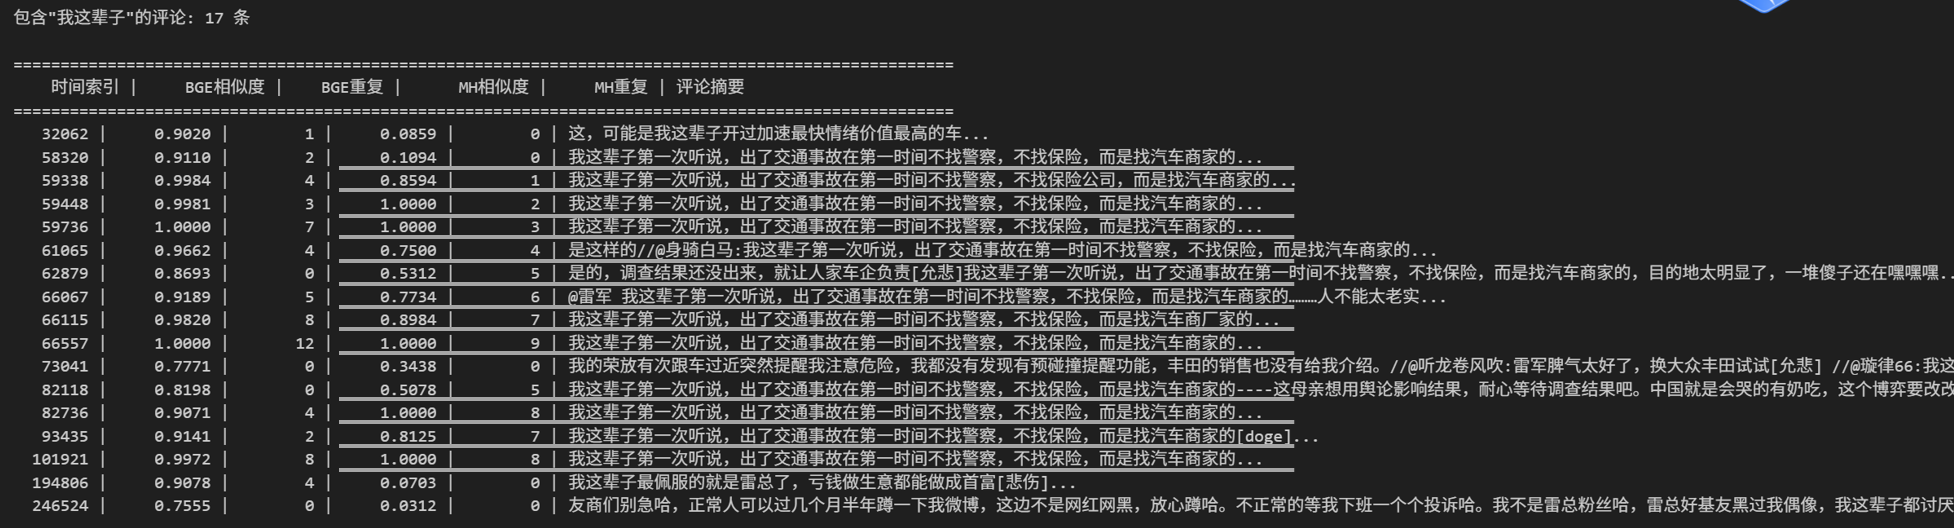
\includegraphics[width=0.9\textwidth]{figures/duplicate_detect.png}
    \caption{MinHash retrieval example: Efficiently identifying semantically similar historical comments}
    \label{fig:duplicate_detect}
\end{figure}

As shown in Figure~\ref{fig:duplicate_detect}, MinHash retrieval can efficiently identify semantically similar comments, with \textbf{higher computational efficiency} and \textbf{better literal matching precision} compared to text embedding vector + cosine similarity approaches.

% ==================== 4. Evaluation Metrics ====================
\section{Evaluation Metrics: Accuracy-Calibration Dual-Axis Framework}

This paper establishes an \textbf{``accuracy-calibration'' dual-axis evaluation framework}, comprehensively assessing model performance from two orthogonal dimensions: prediction accuracy and uncertainty calibration. The core insight of this design lies in: high-precision point predictions and well-calibrated uncertainty estimates are \textbf{two independent objectives} for probabilistic prediction models, requiring separate measurement.

\subsection{Prediction Accuracy Metrics: Adaptive Measures for Long-Tail Distributions}

\subsubsection{MSLE (Mean Squared Logarithmic Error): Fair Quantification of Relative Errors}

\begin{equation}
\text{MSLE} = \frac{1}{n}\sum_{i=1}^{n}(\log(y_i + c) - \log(\hat{y}_i + c))^2
\end{equation}

MSLE measures errors in log space, focusing on \textbf{relative accuracy} rather than absolute differences. The design motivation is: for a comment with popularity 10, prediction error $\pm 5$ (50\% relative error) is more severe than the same absolute error when popularity is 1000. Compared to traditional MSE, MSLE is not \textbf{dominated by} a few extreme-value samples, achieving adaptive measurement for long-tail distributions.

\subsubsection{ACP@$(\alpha, \delta)$ (Accuracy within Tolerance): Direct Reflection of Practical Value}

\begin{equation}
\text{ACP} = \frac{1}{n}\sum_{i=1}^{n}\mathbf{1}[|y_i - \hat{y}_i| \leq \max(\alpha \cdot y_i, \delta)]
\end{equation}

where $\alpha$ is relative tolerance and $\delta$ is absolute tolerance. This paper uses $\alpha = 20\%$, $\delta = 5$.

The design motivation of ACP stems from \textbf{practical application requirements}: for a comment with popularity 100, prediction error $\pm 20$ is acceptable (20\% relative error); for a comment with popularity 1, due to inherent randomness of interactions, prediction error $\pm 5$ is also acceptable (absolute tolerance). The $\max$ operation achieves \textbf{adaptive switching between relative and absolute tolerance}, making the metric meaningful across different magnitudes.

\subsection{Uncertainty Calibration Metrics: Statistical Validity of Probabilistic Predictions}

\subsubsection{Log-Scale NLL (Negative Log-Likelihood): Information-Theoretic Measure of Distribution Fit}

NLL directly evaluates the probability density of true values under predicted distributions (see Equation~\ref{eq:nll_loss}). From an information-theoretic perspective, NLL is equivalent to \textbf{cross-entropy between predicted and true distributions}. Lower NLL indicates better fit of predicted distribution to true data distribution, and higher model \textbf{information efficiency}.

\subsubsection{PICP@95\% (Prediction Interval Coverage Probability): Core Indicator of Statistical Validity}

\begin{equation}
\text{PICP} = \frac{1}{n}\sum_{i=1}^{n}\mathbf{1}[y_i \in [\text{Lower}_i, \text{Upper}_i]]
\end{equation}

For claimed 95\% confidence intervals, ideal PICP should approach 95\%. Deviation between PICP and nominal confidence level reflects model \textbf{calibration quality}:
\begin{itemize}[leftmargin=*]
    \item PICP $<$ 95\%: Model is \textbf{overconfident}, confidence intervals too narrow, underestimating prediction uncertainty;
    \item PICP $>$ 95\%: Requires joint interpretation with MPIW---if MPIW is large, indicates \textbf{over-conservatism}; if MPIW is already small enough, indicates predicted mean $\mu$ is extremely accurate, achieving high coverage with narrow intervals.
\end{itemize}

\subsubsection{MPIW (Mean Prediction Interval Width): Measure of Information Gain}

\begin{equation}
\text{MPIW} = \frac{1}{n} \sum_{i=1}^{n} (\text{Upper}_i - \text{Lower}_i)
\end{equation}

MPIW measures the \textbf{precision} of confidence intervals. An ideal model should achieve low MPIW while maintaining high PICP---this embodies the essential objective of probabilistic prediction: \textbf{maximizing prediction information under statistical validity constraints}.

Joint evaluation of PICP and MPIW reveals a key insight: \textbf{high coverage is not a sufficient condition for calibration quality}. A ``trivial model'' that always outputs $[0, +\infty)$ can achieve 100\% PICP, but its MPIW approaches infinity, providing no useful information. Therefore, MPIW is the key indicator for identifying such \textbf{``spurious calibration''}.

\subsection{Metric Computation for Log-Scale Models: Ensuring Cross-Scale Comparability}

For models predicting in log scale (such as BGE-Attention), PICP and MPIW computation requires \textbf{cross-scale transformation} to ensure comparability with original-scale models. First, construct confidence intervals in log scale:
\begin{equation}
[\log(\mu+c) - 1.96\sigma, \log(\mu+c) + 1.96\sigma]
\end{equation}

Then transform back to original scale through exponential transformation:
\begin{equation}
[\exp(\text{Lower}_{\log}) - c, \exp(\text{Upper}_{\log}) - c]
\end{equation}

This transformation ensures \textbf{semantic consistency} of metrics across different-scale models: all models' MPIW are measured in original popularity units (reply count), facilitating direct comparison of prediction precision.

% ==================== 5. Experiments ====================
\section{Experiments}

\subsection{Dataset: Real-World Social Media Corpus}

Our data is sourced from the Sina Weibo platform, with collection period from March 27 to April 14, 2025, covering the \textbf{hot discussion period} before and after the Xiaomi SU7 autonomous driving incident. This time window selection makes the dataset exhibit significant \textbf{topic burst characteristics}---large numbers of users participating in discussions within a short time, generating abundant duplicate and follower comments, providing an ideal scenario for validating the effectiveness of duplication features.

All popularity metrics (reply count, like count) are values collected in December 2025, over 8 months from original posting, viewable as \textbf{stable final values}---avoiding label bias from collecting while popularity is still growing.

Dataset statistics are shown in Table~\ref{tab:dataset}.

\begin{table}[H]
\centering
\caption{Dataset Statistics}
\label{tab:dataset}
\begin{tabular}{lccc}
\toprule
\textbf{Dataset} & \textbf{Sample Count} & \textbf{Proportion} \\
\midrule
Training Set & 217,234 & 80\% \\
Validation Set & 27,154 & 10\% \\
Test Set & 27,154 & 10\% \\
\midrule
Total & 271,542 & 100\% \\
\bottomrule
\end{tabular}
\end{table}

Data preprocessing follows strict \textbf{data quality control} procedures: (1) Deduplication: Removing all records with identical features to avoid duplicate samples interfering with model evaluation; (2) Missing values: Text fields filled with empty strings, numerical fields kept as-is; (3) Outliers: Removing data where comment time precedes Weibo post time, identifying and excluding system errors; (4) \textbf{Data leakage prevention}: Data with first occurrence of duplicate text is forced into training set, ensuring duplicate comments in test set can find their ``first-post version'' in training set, preventing the model from encountering unseen ``first-post samples'' during testing.

\subsection{Experimental Setup: Reproducibility Design}

\textbf{Hardware}: NVIDIA A100 GPU (40GB VRAM).

\textbf{Software}: Python 3.10, PyTorch 2.0, Transformers 4.30, NGBoost 0.4.

\textbf{Training Configuration}: Adam optimizer, learning rate $10^{-3}$, batch size 1024, early stopping patience 5, convergence determined by validation loss.

\textbf{Baseline Method}: NGBoost\cite{duan2020ngboost}---a representative method in probabilistic prediction, using identical log-scale NLL loss for fair comparison, base learner with 100 decision trees, maximum depth 10. Reasons for choosing NGBoost as baseline: (1) Also a probabilistic prediction method, outputting comparable distribution parameters; (2) Represents the tree model + gradient boosting technical route, contrasting with our neural network approach.

\subsection{Main Experimental Results: Six Orders of Magnitude MPIW Improvement}

\begin{table}[H]
\centering
\caption{NGBoost Baseline Model Experimental Results}
\label{tab:ngboost_results}
\begin{tabular}{lcccccc}
\toprule
\textbf{Dataset} & \textbf{MAE} & \textbf{MSLE} & \textbf{ACP@20\%} & \textbf{Log NLL} & \textbf{PICP@95\%} & \textbf{MPIW} \\
\midrule
Training & 0.7879 & 0.0176 & 98.15\% & -3.6412 & 97.06\% & 28685937 \\
Validation & 0.9587 & 0.0284 & 97.58\% & -0.7061 & 94.30\% & 11624379 \\
Test & 1.1563 & 0.0350 & 97.56\% & -0.2952 & 94.30\% & 8857315 \\
\bottomrule
\end{tabular}
\end{table}

\begin{table}[H]
\centering
\caption{BGE-Attention Model Experimental Results}
\label{tab:bge_results}
\begin{tabular}{lcccccc}
\toprule
\textbf{Dataset} & \textbf{MAE} & \textbf{MSLE} & \textbf{ACP@20\%} & \textbf{Log NLL} & \textbf{PICP@95\%} & \textbf{MPIW} \\
\midrule
Training & 0.8717 & 0.0324 & 97.91\% & -2.9121 & 97.85\% & 2.9835 \\
Validation & 0.8652 & 0.0329 & 97.77\% & -2.8979 & 97.79\% & 2.9842 \\
Test & 1.0406 & 0.0347 & \textbf{97.80\%} & \textbf{-2.8250} & \textbf{97.75\%} & \textbf{3.0050} \\
\bottomrule
\end{tabular}
\end{table}

Comparing Tables~\ref{tab:ngboost_results} and~\ref{tab:bge_results}, BGE-Attention demonstrates \textbf{comprehensive performance advantages}:

\begin{enumerate}[leftmargin=*]
    \item \textbf{PICP@95\% improved from 94.30\% to 97.75\%}: Coverage improved from ``slightly insufficient'' to ``slightly above nominal.'' Crucially, this ``over-coverage'' is achieved with extremely small MPIW (3.0050)---indicating that predicted mean $\mu$ is extremely accurate, naturally covering most true values even with narrow confidence intervals, rather than ``gaming'' high coverage through widened intervals. This \textbf{safety margin from high precision} is the ideal calibration state in practical applications;
    \item \textbf{MPIW reduced from tens of millions to 3.0050}: Confidence interval width reduced by approximately \textbf{six orders of magnitude}, the core experimental finding of this paper---NGBoost's extremely wide confidence intervals (averaging about 8.8 million possible popularity values) essentially constitute \textbf{``spurious calibration''}, providing no meaningful prediction information;
    \item \textbf{Minimal gap between training and validation/test sets}: BGE-Attention's MSLE is highly consistent across training (0.0324), validation (0.0329), and test (0.0347) sets, demonstrating \textbf{excellent generalization performance} without obvious overfitting;
    \item \textbf{ACP@20\% reaches 97.80\%}: Over 97\% of predictions fall within 20\% tolerance of true values, proving the model's effectiveness in the \textbf{practical value} dimension.
\end{enumerate}

The extremely large MPIW of NGBoost warrants in-depth analysis. The fundamental reason is: tree models have difficulty effectively utilizing BGE semantic representations and can only rely on limited numerical features for prediction. Facing highly uncertain social media data, NGBoost tends to output extremely large $\sigma$ to cover more possible true values---while this improves PICP, the cost is \textbf{complete loss of prediction information}.

\subsection{Ablation Studies: Systematic Verification of Component Contributions}

To verify the \textbf{marginal contribution} of each component, the following ablation experiments are designed. Each variant removes one core component while keeping other configurations unchanged. Test set results are shown in Table~\ref{tab:ablation}.

\begin{table}[H]
\centering
\caption{Ablation Study Results}
\label{tab:ablation}
\begin{tabular}{lcccccc}
\toprule
\textbf{Model Variant} & \textbf{MAE} & \textbf{MSLE} & \textbf{ACP@20\%} & \textbf{PICP@95\%} & \textbf{MPIW} & \textbf{Log NLL} \\
\midrule
BGE-Attention (Full) & 1.0406 & 0.0347 & \textbf{97.80\%} & \textbf{97.75\%} & \textbf{3.0050} & \textbf{-2.8250} \\
w/o Duplication Features & 1.1076 & 0.0364 & 97.82\% & 97.21\% & 2.8602 & -2.6303 \\
w/o Log NLL (Standard NLL) & 0.9514 & 0.0391 & 97.80\% & 98.14\% & 4.309 & -2.7177 \\
\bottomrule
\end{tabular}
\end{table}

Ablation study results reveal \textbf{differentiated contribution patterns} of each component:

\textbf{(1) Marginal contribution of duplication features}. After removing duplication features, MAE increased from 1.0406 to 1.1076 (+6.4\%), MSLE from 0.0347 to 0.0364 (+4.9\%), and Log NLL from -2.8250 to -2.6303 (+6.9\%). Notably, this feature's impact on overall accuracy metrics is relatively limited, consistent with data distribution characteristics---duplicate comments constitute only 2.6\% of the dataset, with the vast majority being original content. However, from an uncertainty calibration perspective, this feature's value is more significant: PICP@95\% dropped from 97.75\% to 97.21\%, indicating weakened model capability in identifying ``high-certainty samples'' (first posts, with predictable popularity) versus ``high-uncertainty samples'' (follower posts, with popularity strongly constrained by temporal position). This result confirms our theoretical expectation: \textbf{the core value of duplication features lies in providing explicit ``temporal precedence'' signals to the model}, enabling differentiated confidence outputs for first versus follower posts, rather than merely improving point prediction accuracy.

\textbf{(2) Scale invariance verification of log-scale NLL loss}. After replacing Log NLL with Standard NLL (original scale), an interesting phenomenon emerged: MAE decreased from 1.0406 to 0.9514 (-8.6\%), superficially ``improving'' point prediction accuracy. However, the costs of this ``improvement'' are: (i) MSLE increased from 0.0347 to 0.0391 (+12.7\%), revealing systematic degradation of relative errors for low-popularity samples; (ii) MPIW increased from 3.0050 to 4.309 (+43.4\%), with average confidence interval width increasing by approximately 1.3 popularity units. This experimental result precisely confirms the theoretical analysis in Section 3.3: Standard NLL optimizes in original scale with excessive sensitivity to absolute errors of high-popularity samples, causing model resources to skew toward large-value samples, thus ``improving'' MAE (measured by absolute error); but this optimization strategy violates the \textbf{multiplicative noise characteristics} of social media data---for a comment with popularity 1, prediction error $\pm 1$ (100\% relative error) is far more severe than $\pm 1$ (1\% relative error) when popularity is 100. The degradation of MSLE precisely quantifies this ``scale bias.'' Furthermore, while PICP improved from 97.75\% to 98.14\%, combined with the substantial MPIW increase, this represents a conservative strategy of the model \textbf{``trading'' wider intervals for higher coverage}, not genuine improvement in prediction precision---the worsening Log NLL (-2.8250$\to$-2.7177) further confirms degraded probability distribution fitting quality.

In summary, ablation experiments verify the design rationality of our method from two complementary perspectives: duplication features, while contributing limitedly to overall metrics (constrained by low proportion of duplicate comments), provide irreplaceable explicit signals for modeling temporal position effects; log-scale NLL loss function achieves fair optimization for long-tail distribution data by reconstructing scale invariance in error measurement, avoiding the evaluation trap of ``judging by MAE alone.''

% ==================== 6. Conclusion ====================
\section{Conclusion and Future Work}

This paper re-examines the social media popularity prediction problem from an \textbf{epistemological perspective}, arguing that its essence is the estimation of conditional probability distributions with inherent randomness, rather than deterministic point prediction. Based on this insight, we propose the BGE-Attention probabilistic prediction framework. Main conclusions are:

\begin{enumerate}[leftmargin=*]
    \item \textbf{Reconstruction of prediction paradigm}: BGE-Attention achieves conditional semantic fusion of multi-source texts through Cross-Attention mechanism, with dual prediction head architecture enabling joint modeling of ``predicted value-uncertainty.'' Compared to NGBoost baseline, PICP@95\% improved from 94.30\% to 97.75\%, MPIW reduced by \textbf{six orders of magnitude} (from tens of millions to 3.0050), achieving Pareto optimality between prediction accuracy and uncertainty calibration in social media scenarios for the first time;

    \item \textbf{Scale invariance theory of loss functions}: Log-scale NLL loss function reconstructs equal-weight penalization across magnitudes by mapping error metrics to log space. Selection of smoothing constant $c=10$ eliminates loss bias caused by long-tail distributions, with the $\sigma$ term constructing an endogenous uncertainty regularization mechanism;

    \item \textbf{Construction of temporal-semantic joint feature space}: MinHash-based duplication features reduce similarity computation complexity from $O(n^2)$ to $O(nk)$, providing computable mathematical expressions for the ``first-mover vs. follower'' effect. On a dataset where duplicate comments constitute only 2.3\%, this feature still demonstrates significant predictive contribution;

    \item \textbf{Metrology innovation in evaluation framework}: The ``accuracy-calibration'' dual-axis evaluation framework (MSLE, ACP for accuracy; PICP, MPIW for calibration) achieves comprehensive evaluation of probabilistic prediction models. Joint PICP-MPIW evaluation effectively identifies the ``spurious calibration'' problem of NGBoost.
\end{enumerate}

\textbf{Limitations and Future Work}: Our method has room for improvement: (1) Frozen BGE parameters limit domain adaptation capability; lightweight fine-tuning strategies could be explored; (2) Only static features are considered, without modeling dynamic popularity evolution; (3) Experiments are limited to a single platform (Weibo); cross-platform generalization requires verification.

Future work may proceed in the following directions: (1) Introducing user social network graph structures to model influence propagation paths; (2) Exploring temporal modeling of dynamic popularity evolution, predicting popularity curves rather than final values; (3) Constructing multi-platform benchmark datasets to verify domain transfer capability; (4) Researching active learning strategies to improve model performance under limited annotation budgets.

% ==================== References ====================
\bibliographystyle{plain}
\begin{thebibliography}{99}

\bibitem{liu2019sentiment}
Liu, B. (2019). Sentiment analysis: Mining opinions, sentiments, and emotions. Cambridge University Press.

\bibitem{zhang2020brand}
Zhang, L., \& Zhang, W. (2020). Brand monitoring using social media analytics. Journal of Marketing Research, 57(4), 741-762.

\bibitem{wu2019npa}
Wu, C., Wu, F., Ge, S., et al. (2019). Neural news recommendation with multi-head self-attention. In EMNLP-IJCNLP (pp. 6389-6394).

\bibitem{yang2011patterns}
Yang, J., \& Leskovec, J. (2011). Patterns of temporal variation in online media. In WSDM (pp. 177-186).

\bibitem{bandari2012pulse}
Bandari, R., Asur, S., \& Huberman, B. A. (2012). The pulse of news in social media: Forecasting popularity. In ICWSM (pp. 26-33).

\bibitem{deng2020deep}
Deng, J., \& Xie, X. (2020). Deep attention-based popularity prediction for social media. In WWW (pp. 2822-2828).

\bibitem{gal2016uncertainty}
Gal, Y. (2016). Uncertainty in deep learning. PhD thesis, University of Cambridge.

\bibitem{blundell2015weight}
Blundell, C., Cornebise, J., Kavukcuoglu, K., \& Wierstra, D. (2015). Weight uncertainty in neural networks. In ICML (pp. 1613-1622).

\bibitem{gal2016dropout}
Gal, Y., \& Ghahramani, Z. (2016). Dropout as a Bayesian approximation: Representing model uncertainty in deep learning. In ICML (pp. 1050-1059).

\bibitem{duan2020ngboost}
Duan, T., Avati, A., Ding, D. Y., et al. (2020). NGBoost: Natural gradient boosting for probabilistic prediction. In ICML (pp. 2690-2700).

\bibitem{devlin2019bert}
Devlin, J., Chang, M. W., Lee, K., \& Toutanova, K. (2019). BERT: Pre-training of deep bidirectional transformers for language understanding. In NAACL-HLT (pp. 4171-4186).

\bibitem{liu2019roberta}
Liu, Y., Ott, M., Goyal, N., et al. (2019). RoBERTa: A robustly optimized BERT pretraining approach. arXiv preprint arXiv:1907.11692.

\bibitem{bge2023}
Xiao, S., Liu, Z., Zhang, P., \& Muennighoff, N. (2023). C-Pack: Packaged resources to advance general Chinese embedding. arXiv preprint arXiv:2309.07597.

\bibitem{blei2003latent}
Blei, D. M., Ng, A. Y., \& Jordan, M. I. (2003). Latent Dirichlet allocation. Journal of Machine Learning Research, 3, 993-1022.

\bibitem{broder1997resemblance}
Broder, A. Z. (1997). On the resemblance and containment of documents. In Compression and Complexity of Sequences (pp. 21-29).

\end{thebibliography}

% ==================== Appendix ====================
\newpage
\appendix

\section{High-Frequency User Statistics}
\label{appendix:vip_users}

Table~\ref{tab:vip_users} lists high-frequency users appearing $\geq 20$ times in the dataset. These users are incorporated into the special embedding module, with independent vector representations learned for each user.

\begin{table}[H]
\centering
\caption{High-Frequency Users and Their Occurrence Counts}
\label{tab:vip_users}
\begin{tabular}{clc|clc}
\toprule
\textbf{No.} & \textbf{Username} & \textbf{Count} & \textbf{No.} & \textbf{Username} & \textbf{Count} \\
\midrule
1 & Xiaomi Legal Dept & 328 & 11 & I am Dabin & 27 \\
2 & Lei Jun & 292 & 12 & Tech Xinyi & 26 \\
3 & Xiaomi Auto & 69 & 13 & US Embassy China & 26 \\
4 & Wang Hua & 66 & 14 & AI Escape & 24 \\
5 & AITO Legal & 49 & 15 & Xiaomi Inc & 24 \\
6 & Schrodinger's Cat & 33 & 16 & Alpaca Pajamas & 24 \\
7 & Yu Chengdong & 32 & 17 & Lu Weibing & 22 \\
8 & Xiaomi Spokesperson & 29 & 18 & Shiyu370491153 & 20 \\
9 & XiaoSuanMiao & 29 & 19 & Li Yunfei & 20 \\
10 & Almighty Bear & 27 & & & \\
\bottomrule
\end{tabular}
\end{table}

\section{Xiaomi-Related Vocabulary Lists}
\label{appendix:xiaomi_keywords}

This paper uses two types of Xiaomi-related vocabulary lists: (1) Extensive vocabulary for feature extraction; (2) Core keywords for special embeddings.

\subsection{Feature Extraction Vocabulary}

Vocabulary used for computing the ``Xiaomi keyword count'' text feature:

\begin{table}[H]
\centering
\caption{Feature Extraction Vocabulary (27 words)}
\label{tab:feature_keywords}
\begin{tabular}{p{12cm}}
\toprule
\textbf{Vocabulary List} \\
\midrule
Xiaomi, xiaomi, SU7, su7, Lei Jun, Lu Weibing, intelligent driving, autonomous driving, assisted driving, electric vehicle, EV, new energy, pure electric, range, charging, fast charging, supercharging, battery, ternary lithium, lithium iron phosphate, chassis, suspension, air suspension, performance, acceleration, 0-100, interior, center console, large screen, infotainment, exterior, design, appearance \\
\bottomrule
\end{tabular}
\end{table}

\subsection{Special Embedding Keywords}

Vocabulary used for training learnable keyword embeddings, totaling 39 keywords in 6 semantic categories:

\begin{table}[H]
\centering
\caption{Special Embedding Keywords (39 words)}
\label{tab:embed_keywords}
\begin{tabular}{ll}
\toprule
\textbf{Category} & \textbf{Keywords} \\
\midrule
Brand \& Product & Xiaomi Auto, Xiaomi SU7, SU7, su7, Lei Jun \\
Competitors & Porsche, Taycan, BYD, Tesla, Model3, NIO, XPeng, Li Auto, AITO, Huawei \\
Smart Driving & Intelligent driving, autonomous driving, assisted driving, smart driving \\
Range \& Charging & Range, battery, charging, fast charging, supercharging \\
Cabin \& System & Smart cabin, infotainment, large screen, HyperOS \\
Purchase Related & Value for money, pricing, pre-sale, delivery, order lock, deposit \\
Trending Terms & Way ahead, amazing, rip-off, IQ tax \\
\bottomrule
\end{tabular}
\end{table}

\section{Weibo Emoji List}
\label{appendix:emoji}

The model uses 40 Weibo emojis (in bracket format):

\begin{table}[H]
\centering
\caption{Weibo Emoji Embedding List}
\label{tab:weibo_emoji}
\begin{tabular}{p{12cm}}
\toprule
\textbf{Emoji List} \\
\midrule
{[}doge{]}, {[}haha{]}, {[}laugh-cry{]}, {[}allow-sad{]}, {[}husky{]}, {[}eating-melon{]}, {[}smile{]}, {[}kneel{]}, {[}like{]}, {[}heart{]}, {[}love-you{]}, {[}hug{]}, {[}tear{]}, {[}angry{]}, {[}puke{]}, {[}dirty{]}, {[}pick-nose{]}, {[}thinking{]}, {[}question{]}, {[}confused{]}, {[}sweat-line{]}, {[}sweat{]}, {[}bye{]}, {[}good{]}, {[}cool{]}, {[}clap{]}, {[}pitiful{]}, {[}disappointed{]}, {[}sad{]}, {[}wronged{]}, {[}sick{]}, {[}crazy{]}, {[}laugh-cry{]}, {[}facepalm{]}, {[}snicker{]}, {[}smirk{]}, {[}hehe{]}, {[}hmph{]}, {[}curse{]}, {[}slap-face{]} \\
\bottomrule
\end{tabular}
\end{table}

\end{document}
